\documentclass{beamer}\usepackage{graphicx, color}
%% maxwidth is the original width if it is less than linewidth
%% otherwise use linewidth (to make sure the graphics do not exceed the margin)
\makeatletter
\def\maxwidth{ %
  \ifdim\Gin@nat@width>\linewidth
    \linewidth
  \else
    \Gin@nat@width
  \fi
}
\makeatother

\IfFileExists{upquote.sty}{\usepackage{upquote}}{}
\definecolor{fgcolor}{rgb}{0.2, 0.2, 0.2}
\newcommand{\hlnumber}[1]{\textcolor[rgb]{0,0,0}{#1}}%
\newcommand{\hlfunctioncall}[1]{\textcolor[rgb]{0.501960784313725,0,0.329411764705882}{\textbf{#1}}}%
\newcommand{\hlstring}[1]{\textcolor[rgb]{0.6,0.6,1}{#1}}%
\newcommand{\hlkeyword}[1]{\textcolor[rgb]{0,0,0}{\textbf{#1}}}%
\newcommand{\hlargument}[1]{\textcolor[rgb]{0.690196078431373,0.250980392156863,0.0196078431372549}{#1}}%
\newcommand{\hlcomment}[1]{\textcolor[rgb]{0.180392156862745,0.6,0.341176470588235}{#1}}%
\newcommand{\hlroxygencomment}[1]{\textcolor[rgb]{0.43921568627451,0.47843137254902,0.701960784313725}{#1}}%
\newcommand{\hlformalargs}[1]{\textcolor[rgb]{0.690196078431373,0.250980392156863,0.0196078431372549}{#1}}%
\newcommand{\hleqformalargs}[1]{\textcolor[rgb]{0.690196078431373,0.250980392156863,0.0196078431372549}{#1}}%
\newcommand{\hlassignement}[1]{\textcolor[rgb]{0,0,0}{\textbf{#1}}}%
\newcommand{\hlpackage}[1]{\textcolor[rgb]{0.588235294117647,0.709803921568627,0.145098039215686}{#1}}%
\newcommand{\hlslot}[1]{\textit{#1}}%
\newcommand{\hlsymbol}[1]{\textcolor[rgb]{0,0,0}{#1}}%
\newcommand{\hlprompt}[1]{\textcolor[rgb]{0.2,0.2,0.2}{#1}}%

\usepackage{framed}
\makeatletter
\newenvironment{kframe}{%
 \def\at@end@of@kframe{}%
 \ifinner\ifhmode%
  \def\at@end@of@kframe{\end{minipage}}%
  \begin{minipage}{\columnwidth}%
 \fi\fi%
 \def\FrameCommand##1{\hskip\@totalleftmargin \hskip-\fboxsep
 \colorbox{shadecolor}{##1}\hskip-\fboxsep
     % There is no \\@totalrightmargin, so:
     \hskip-\linewidth \hskip-\@totalleftmargin \hskip\columnwidth}%
 \MakeFramed {\advance\hsize-\width
   \@totalleftmargin\z@ \linewidth\hsize
   \@setminipage}}%
 {\par\unskip\endMakeFramed%
 \at@end@of@kframe}
\makeatother

\definecolor{shadecolor}{rgb}{.97, .97, .97}
\definecolor{messagecolor}{rgb}{0, 0, 0}
\definecolor{warningcolor}{rgb}{1, 0, 1}
\definecolor{errorcolor}{rgb}{1, 0, 0}
\newenvironment{knitrout}{}{} % an empty environment to be redefined in TeX

\usepackage{alltt}
\usetheme{Stats}
\setbeamercovered{transparent}
\usepackage{color}
\usepackage{hyperref}
  \hypersetup{
  	colorlinks=true
		linkcolor=black
		}
\usepackage{url}
\usepackage{graphics}
\usepackage{tikz}
\usepackage{booktabs}





%%%%%%%%%%%%%%%%%%%%%%%%%%%%%%%% Title Slide %%%%%%%%%%%%%%%%%%%%%%%%%%
\title[]{Intro to Social Science Data Analysis \\[1cm] Week 11 Seminar: Simple Linear Regression}
\author[]{
    \href{mailto:gandrud@yonsei.ac.kr}{Christopher Gandrud}
}
\date{\today}


\begin{document}

\frame{\titlepage}

\frame{
  \frametitle{Interpretation}
  With a partner, 
  \begin{itemize}
      \item<1-> describe the relationship between the number of calories a food item has and its carbohydrates,
      \item<1-> roughly estimate how many carbohydrates an item with 300 calories would have,
      \item<1-> what are the independent and dependent variables?
  \end{itemize}
  \begin{center}
    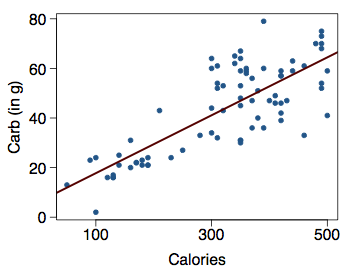
\includegraphics[scale=0.5]{CalCarb.png}
  \end{center}
}

\frame{
  \frametitle{Outliers}
  This graph plots states in the United States. \\
  The outlier on the bottom right is Washington, DC. \\
  What should we do with the outlier?
  \begin{center}
    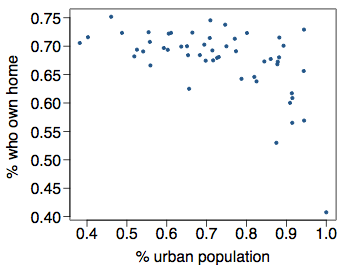
\includegraphics[scale=0.5]{Outlier.png}
  \end{center}
}

\frame{
	\frametitle{Inference from Intercepts}
  What does the point estimate of $\alpha$ mean?\\[0.5cm]
  How interested are we in making inferences from $\hat{\alpha}$?
}

\frame{
  \frametitle{Interpreting Dummy Variables}
  The variable \texttt{Elect} is a dummy variable equalling 1 when a country has an elected legislature and 0 when it does not. \\[0.5cm]
  Predict its \texttt{GDPperCapita} in thousands of US dollars for countries with and without elected legislatures using the following simple linear regression equation:
  \[
  \tt{GDPperCapita} = 12 + 14(\tt{Elect})
  \]\\[0.5cm]
  Note: this is not based on real data.
}


\begin{frame}[fragile]
  \frametitle{Load Data}
  Load data on 3143 US counties from the {\emph{openintro}} package.
\begin{knitrout}
\definecolor{shadecolor}{rgb}{0.969, 0.969, 0.969}\color{fgcolor}\begin{kframe}
\begin{alltt}
\hlcomment{# Load library}
\hlfunctioncall{library}(openintro)

\hlcomment{# Load Data}
\hlfunctioncall{data}(county)

\hlcomment{# Show variable names}
\hlfunctioncall{names}(county)
\end{alltt}
\begin{verbatim}
##  [1] "name"          "state"        
##  [3] "pop2000"       "pop2010"      
##  [5] "fed_spend"     "poverty"      
##  [7] "homeownership" "multiunit"    
##  [9] "income"        "med_income"
\end{verbatim}
\end{kframe}
\end{knitrout}

\end{frame}

\frame{
  \frametitle{Practice}
  Pick two continuous variables. Explore the relationship between the variables, including:
  \begin{itemize}
  \item their correlation,
  \item the direction of the relationship, 
  \item the strength of the relationship,
  \item predict three values of one variable based on three values of the other,
  \item statistical inferences from a linear regression equation.
\end{itemize} \\[0.5cm]
  Could the two variables be causally related? Why/why not?
}


\end{document}
